\chapter{Stand der Technik, Process Mining im Smart Home}\label{chap:stateoftheart}

Generell beschäftigt sich Process Mining mit der Aufgabe, Modelle von realen Prozessen, im Gegensatz zu solchen die von Betrachtern vermutet oder angenommen werden, mit Hilfe von Ereignisprotokollen zu extrahieren, diese zu vergleichen und zu optimieren.\cite{PMinAction}
Dieser Extraktionsprozess von formalisiertem Prozesswissen aus Eventlogs heraus kann in den  unterschiedlichsten Anwendungsgebieten eingesetzt werden, um neue Erkenntnisse über komplexe Abläufe zu erhalten. 

Während der Einsatz in Smart Living Szenarien bisher nur in Ansätzen erforscht wurde, kommt Process Mining in Unternehmen bereits häufiger zum Einsatz, Vgl.\cite{litreview}.

\section{Process Mining im Kontext der Business Analytics und Business Intelligence}

Die Digitalisierung in der Industrie macht durch die gesteigerte Verbreitung von vernetzten Endgeräten rasante Fortschritte und legt dadurch auch das Fundament für die Auswertung großer Datenmengen, in denen Informationen über Prozessabläufe eingebettet sind, Vgl. \cite{GanscharGerlac}. 

In der IT Architektur zahlreicher Unternehmen trifft man häufig auf dezentrale, verteilte technologische Systeme, in denen die unterschiedlichen technologischen Komponenten isoliert, häufig auch als Service eines Drittanbieters, vorliegen , Vgl.\cite{GanscharGerlac}. Dies hat zur Folge, dass an einem einzelnen Prozess unterschiedliche Module, wie das ERP- (Enterprise Ressource Planing), CRM- (Customer Relationship Management) oder SCM-System (Supply Chain Management), beteiligt sind, welche jeweils ihre eigene Informationen zu einem relevanten Prozessablauf bereitstellen. Process Mining kann an dieser Stelle einen entscheidenden Beitrag dazu leisten, festzustellen, ob die internen Abläufe geplanten Prozessen entsprechen und an welchen Stellen diese sich verbessern ließen, Vgl.\cite{PMinAction}.

Process Mining ist außerdem in der Lage Informationen über einen Prozess zu extrahieren, unabhängig davon ob seine Struktur den Teilnehmern des Prozesses oder seinen Organisatoren bekannt ist. Gegenteilig dazu muss bei der Business Process Analysis oder bei dem Business Activity Monitoring zunächst auf a-priori bekannte Geschäftsprozesse zurückgegriffen werden, um diese anschließend zu analysieren. 

Process Mining umfasst dabei nicht allein die Analyse von Abläufen, sondern auch das Entdecken von Zusammenhängen zwischen einzelnen Komponenten und ihren Aktivitäten. Dadurch erübrigt sich bei korrekter Anwendung von Process Mining zur Arbeitsprozessmodellierung, beispielsweise innerhalb eines Unternehmens, die Durchführung von Befragungen der Mitarbeiter zu ihrem Arbeitsprozess. Dies hat zum Vorteil, dass der Einfluss von subjektiven Sichten auf das resultierende Modell minimiert wird und bei der Analyse vergleichsweise zeit- und ressourcenschonend vorgegangen werden kann.
\begin{figure}[!ht]
    \centering
    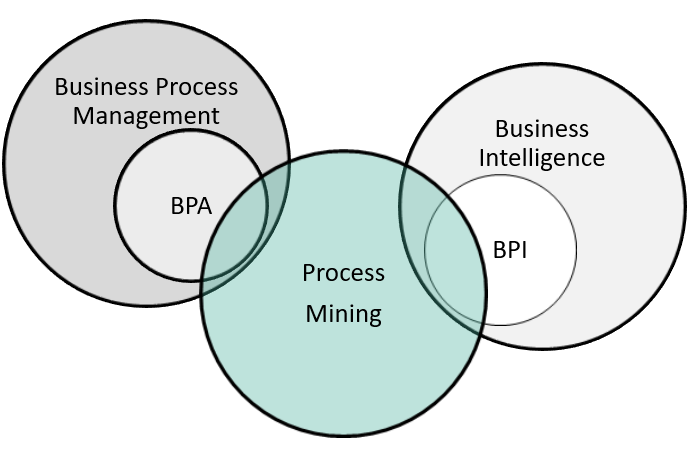
\includegraphics[scale=0.41]{figures/Appbildungen/businessanalytics.PNG}
    \caption{Process Mining im Kontext anderer Verfahren der Unternehmensanalyse,  (Eigene Darstellung in Anlehnung an: Weerdt, J.D., et al., 2013, S.64,\cite{DeWeerdt})}
    \label{fig:BIContext}
\end{figure}

Process Mining kann also als Analysetool, welches sich zwischen der Business Intelligence und dem Business Process Management bewegt, verstanden werden, siehe Abbildung (\ref{fig:BIContext}).

Die Autoren der Metastudie 'Business Process Mining Application: A Literature Review' \cite{litreview} haben aktuelle Veröffentlichungen zum Thema Process Mining auf ihr Anwendungsgebiet hin untersucht und unter anderem herausgefunden, dass in knapp einem Drittel der herangezogenen Literatur Process Mining im Gesundheits- und Pflegedienst eingesetzt worden ist, gefolgt vom IT und Finanzsektor.

\section{Einsatz in der Gesundheits- und Altenpflege}
Eine Studie zum Process Mining in der Geriatrie, die Anfang 2019 im ‚Biomedical Engineering Systems and Technologies Journal‘ erschienen ist \cite{wrro141683}, hat unter allen wissenschaftlichen Veröffentlichungen zum Thema acht Studien identifiziert, die Process Mining erfolgreich in der Altenpflege eingesetzt haben. Bei diesen Studien lag der Fokus nicht allein darauf, einzelne Behandlunsgverläufe und Daten aus den Krankenakten der Patienten systematisch zu analysieren, sondern auch darauf, ihre alltäglichen Handlungensmuster auswerten zu können. 

An dieser Stelle ergibt sich eine Schnittmenge des Process Mining mit dem Forschungsgegenstand der Untersuchung von alltäglichen menschlichen Aktivitäten (englisch \textit{Activities of Daily Living}, kurz ADL). 
Gegenstand einer der einbezogenen Studien war beispielsweise die Pflege von demenzerkrankten Patienten in einem Pfelgeheim, veröffentlicht von Llatas et al. \cite{llatas}, welches mit zahlreichen Sensoren ausgestattet war, deren Eventlogs durch Process Mining ausgewertet wurden. Im Detail wurde hier Conformance Checking eingesetzt. Mithilfe der Auswertung konnten  Differenzen in den Zeitspannen der Alltagsroutinen der untersuchten Patienten beobachtet werden. Eine verlangsamte Routine, oder gravierende Abweichungen zu früheren Tagesabläufen, konnten als frühes Signal einer Veränderung im gesundheitlichen Zustand der Bewohner interpretiert werden.

\section{Process Mining und Menschliches Verhalten}
Anhand solcher Studien wird ersichtlich, dass Process Mining auch dem Forschungsfeld der \textit{Human Activity Recognition}, kurz HAR, dienen kann. HAR beschreibt ein Forschungsfeld, das untersucht wie menschliche Aktivitäten, die mit Sensoren aufgenommen wurden, korrekt klassifiziert und auf ihnen zugrundeliegende Muster hin untersucht werden können. 

Events im Eventlog entstehen dann beispielsweise durch Bewegungssensoren, die im Gebäude verteilt werden, Näherungssensoren in elektrischen Geräten und anderen Zustandssensoren, die je zahlreicher und weiter sie gestreut sind, ein klareres Bild über das Verhalten der beobachteten Personen schaffen können. 
Dieser Aspekt unterscheidet Process Mining im Smart Living Kontext vom Process Mining Einsatz im Unternehmen, wo Logs durch meistens durch die bereits vorhandene IT Technik gespeist werden und selten auf die zusätzliche Anreicherung durch Sensoren angewiesen sind.
 
Im Unterschied zur industriellen Umgebung ist die private menschliche Umgebung außerdem gravierenden Schwankungen unterworfen. Dies ist vor allen Dingen dem Umstand geschuldet, dass Unternehmen intern zunächst Arbeitsprozesse planen, definieren und anschließend umsetzen und dabei darauf fokussiert sind, wenig Spielraum für unerwartete Abweichungen im Arbeitsablauf zuzulassen. 
Wie eine Person privat vernetzte Geräte nutzt ist keinem formalen Regelwerk unterworfen. Ein sogenanntes Smart Home ist deutlich weniger reglementiert als eine Fabrik und jeder Anwender entscheidet individuell darüber, welche IoT Geräte wann Teil seines Smart Home werden. Auf diese Weise entsteht in jedem Eigenheim ein individuelles Geflecht aus vernetzten Sensoren und Aktoren, die meist von unterschiedlichen Herstellern stammen, welche selten alle ein und den selben Standards folgen.

Unternehmensinterne Logs sind aus diesem Grund von Beginn an aussagekräftiger als private. Jeder Eintrag lässt sofort Rückschlüsse über die Semantik und den Kontext des Eintrags zu und ist, auch vom Rest des Logs isoliert, interpretierbar. Währenddessen sind Logs aus privaten Umgebungen auf Metainformationen angewiesen, bevor sie interpretiert werden können und einzelne Einträge eines Logs sind, aus dem Kontext der anderen Geräte in ihrer Umgebung herausgenommen, nicht aussagekräftig Vgl.\cite{Jaroucheh2011}.

Ein entscheidender Vorteil der Auswertung von Eventlogs im Smart Home im Hinblick auf Privatsphäre und Datenschutz jedoch ist, dass sie von den beobachteten Personen eher akzeptiert wird als eine Überwachung durch beispielsweise Videokameras. Im Gegensatz zur Videoüberwachung können Eventlogs direkt zur Auswertung genutzt werden, ohne dabei den Umweg über die Bildanalyse gehen zu müssen, Vgl.\cite{TaxSidorova}.

Zurzeit wird erforscht, wie die Komplexität menschlicher Aktivität durch Algorithmen korrekt erfasst und abstrahiert werden kann. Der Artikel "Discovering more precise process models from event logs by filtering out chaotic activities", der 2018 im Journal of Intelligent Information Systems veröffentlicht wurde, stellt beispielsweise ein Verfahren vor, das Eventlogs aus dem Smart Home effektiver filtern kann, als bisher übliche Algorithmen, so die Autoren \cite{Tax2019}. Ihre Forschung war dadurch motiviert, dass die im Process Mining verbreitete Herangehensweise, häufigkeitsbasierte Schwellwerte zu nutzen, um Rauscheinträge zu filtern, für die Auswertung von Smart Home Daten häufig in nur unzureichende Modellen resultiert. 
Sie stellten vier Filtertechniken für Eventlogs vor, die mit realen Eventlogs, die aus der Industrie und aus dem Smart Home Bereich stammten, untersucht wurden. Die Filter kalkulieren die Relevanz von Einträgen im Eventlog auf der Basis von der Entropie der Eingangsdaten, bayesischer Infernenz und weiteren Faktoren. Die Ergebnisse der Untersuchung haben gezeigt, dass Datensätze, die über die vorgestellten Filtertechniken in den meisten Fällen zu einer präziseren Modellierung führen, als Ausgabemodelle, deren Eingangsdaten nur über Häufigkeitsfilter vorverarbeitet wurden. 

Allerdings zeigte sich auch hier, dass die Auswertung von Protokolldaten aus industriellen Umgebungen deutlich zuverlässigere Ergebnisse liefert, als die Auswertung von Daten aus dem privaten Raum. Auch die verbesserten Filter sind, je nach Beschaffenheit der Eventlogs und der inkonsistenz der Einträge, keine ausreichende Maßnahme gewesen, um sicherzustellen, dass  menschliches Verhalten korrekt abstrahiert wird.

Es wird deutlich, dass Verfahren und Vorverarbeitung von Datensätzen, die für die Analyse von menschlichem Verhalten eingesetzt werden, individuell an das zu beobachtende Szenario angepasst werden müssen und es bisher keine universelle Lösung für die Auswertung von ADL durch Process Mining gibt.

%leads to the highest F-score: on the CHAD event log the indirect activity filter outperforms the direct activity filter when using the Inductive Miner infrequent 20%; however, the direct activity filter leads to higher F-score for the Inductive Miner when filtering more than 50% of the activities. Figure 14 shows the nondeterminism results for the human behavior event logs. It is noticeable that the nondeterminism values of the process models that are discovered when filtering very few activities are much closer to the flower model compared to what we have seen before for the business process event logs. This is caused by human behavior event logs having much more variability in behavior compared to execution data from business processes, resulting in a much harder process discovery task. After filtering several chaotic activities, the nondeterminism drops significantly to ranges comparable to nondeterminism values seen for logs from the business process domain. This shows that the problem of chaotic activities is much more prominent in human behavior event logs than in business process event logs. The entropy-based activity filtering approaches lead to more deterministic process models compared to filtering out infrequent activities

\section{Vor- und Nachbereitung von Datensätzen}
Ähnlich wie bei den meisten Datenanalyse Technologien gilt auch für Process Mining, dass eine komplexe und aussagekräftige Auswertung nicht ohne Vor- und Nachbearbeitung der Daten durchgeführt werden kann.

Die Vorbereitung (oder das Preprocessing) beim Process Mining greift dabei größtenteils die Hindernisse auf, die in Abschnitt \ref{challanges} erläutert wurden. Wie die meisten Datananalysemethoden profitieren auch Process Mining Verfahren davon, wenn Rauschdaten entfernt werden, bevor der Datensatz verarbeitet wird. 

Lassen sich Unterschiede im Format der Einträge verschiedener Ressourcen ausmachen, so ist es notwendig diese in eine einheitliche Form zu überführen, seien es verschiedene Zeitstempfelformattierungen oder unterschiedliche Schreibweisen für identische Abläufe. Je einheitlicher die Form des Logs desto besser wird auch die Qualität der Ausgabe sein, Vgl.\cite{PMinAction}. Ereignislücken sollten wenn möglich geschlossen und Einträge, die fälschlicherweise entstanden sind, bereinigt werden.

Auch die Nachbearbeitung (oder das Postprocessing) ist ein in den meisten Anwendungsfällen unerlässlicher Vorgang, bevor ein  Modell als Ergebnis der Analyse akzeptiert wird. Häufig ergibt sich an dieser Stelle der Datenanalyse eine sogenannte Feedbackloop, das heißt ein Modell wird vom Analyseverfahren generiert. Bevor es zur Interpretation des Sachverhalts freigegeben werden kann wird untersucht, ob Fehler im Modell vorliegen, die dem Analyseverfahren eigen sind und gegen die dann entgegengesteuert werden muss. 

Idealerweise liegt für diesen Schritt beim Analytiker, oder dem Analysesystem, Wissen über die Schwächen des eingesetzten Verfahrens vor. Zuträglich für die Qualität des Modells sind auch Vorabinformationen über die Prozesse, die den Eingangsdaten innewohnen. Dieses Wissen kann genutzt werden, um einzelne Parameter im Verfahren nachzujustieren, die Wahl von Schwellwerten anzupassen, oder größere Datensätze heranzuziehen, um eine höhere Sicherheit hinsichtlich der Korrektheit des resultierenden Modells zu garantieren.

Welche Parameter anpassbar sind und mit welcher Methode effektiv die richtigen Werte gefunden werden können, ist vom Anwendungsfall und den Ansprüchen abhängig, die diejenigen Personen an das Modell haben, die es interpretieren wollen. 

Die Aussagefähigkeit von Ausgabemodellen ist also abhängig von zahlreichen Faktoren wie der eingesetzten Software, dem Analyseverfahren, der Verarbeitung der gesammelten Daten und Datenqualität, sowie der Fragestellung, die durch die Analyse beantwortet werden soll.

Grundsätzlich ist aber festzuhalten, dass der Aufwand des Pre- und Postprocessing umso rapider wächst, je unbeständiger und unregelmäßiger die Abläufe sind, die durch Process Mining evaluiert werden sollen. 

Auf der einen Seite des Spektrums des Bedarfs an Pre- und Postprocessing befinden sich  beispielsweise Automatisierungsanlagen, die einem vordefinierten Ablauf folgen, bis sie durch einen Fehlerfall unterbrochen werden. Diese sind prinzipiell durch ein eindeutiges, wenn nicht zwangsläufig einfaches, Modell abstrahierbar.

Auf der anderen Seite befinden sich ungeordnete Umgebungen die es zu analysieren gilt, wie etwa Personen und ihre Abläufe in einem privaten Raum, deren Prozesse im Detail nur schwer durch Modellierung greifbar sind. 